\documentclass[a4paper,12pt]{article}
\pdfminorversion=7

% =========================================================
% LANGUAGE AND FONT
% =========================================================
\usepackage[english]{babel}
\usepackage[T1]{fontenc}
\usepackage{lmodern}
\usepackage{microtype}
\emergencystretch=2em

% =========================================================
% PAGE LAYOUT
% =========================================================
\usepackage[
    a4paper,
    left=2cm,
    right=2cm,
    top=2.2cm,
    bottom=1.8cm,
    headheight=25pt,
    headsep=11pt,
    footskip=20pt
]{geometry}

\setlength{\parindent}{0.75cm}
\setlength{\parskip}{0.04cm}

% =========================================================
% MATHEMATICS AND ENGINEERING
% =========================================================
\usepackage{mathtools,amsthm,amssymb,dsfont}
\usepackage{siunitx}

\sisetup{
    per-mode=symbol,
    mode=match
}

% =========================================================
% BRAND COLORS (Prover Technology Visual Identity)
% =========================================================
\usepackage[dvipsnames]{xcolor}

\definecolor{ProverMadison}{HTML}{0B3360}     % Primary navy
\definecolor{ProverCornflower}{HTML}{569FF7}  % Secondary blue
\definecolor{ProverButtercup}{HTML}{F4A220}   % Accent gold/orange
\definecolor{ConfRed}{HTML}{C9252B}           % Confidentiality red

\definecolor{SlateText}{HTML}{202B3A}
\definecolor{MutedGray}{HTML}{65748A}
\definecolor{LightGray}{HTML}{E9EDF3}
\definecolor{CodeBg}{HTML}{F8FAFC}

\colorlet{ProverNavy}{ProverMadison}
\colorlet{ProverBlue}{ProverCornflower}

% =========================================================
% FIGURES AND TABLES
% =========================================================
\usepackage{graphicx}
\usepackage{float}
\usepackage{caption}
\usepackage{subcaption}
\usepackage{array}
\usepackage{booktabs}
\usepackage{multirow}
\usepackage{tabularx}
\newcolumntype{Y}{>{\RaggedRight\arraybackslash}X}

\captionsetup[figure]{
    font=small,
    labelfont={bf,color=ProverMadison},
    skip=4pt,
    justification=centering
}
\captionsetup[table]{
    font=small,
    labelfont={bf,color=ProverMadison},
    skip=3pt,
    position=top
}

% =========================================================
% FORMATTING AND SECTION TITLES
% =========================================================
\usepackage{titlesec}
\usepackage{enumitem}
\usepackage{ragged2e}

\setlist{noitemsep,topsep=1.5pt,parsep=0pt,partopsep=0pt}

\titleformat{\section}
    {\normalfont\Large\bfseries\color{ProverMadison}}
    {\thesection}{0.7em}{}
\titlespacing*{\section}{0pt}{8pt plus 1pt minus 1pt}{3pt plus 1pt minus 1pt}

\titleformat{\subsection}
    {\normalfont\large\bfseries\color{ProverMadison}}
    {\thesubsection}{0.7em}{}
\titlespacing*{\subsection}{0pt}{6pt plus 1pt minus 1pt}{2pt plus 1pt minus 1pt}

\titleformat{\subsubsection}
    {\normalfont\normalsize\bfseries\color{ProverMadison!90!black}}
    {\thesubsubsection}{0.7em}{}
\titlespacing*{\subsubsection}{0pt}{4pt plus 1pt minus 1pt}{2pt plus 1pt minus 1pt}

\setcounter{secnumdepth}{3}
\setcounter{tocdepth}{2}

% Inline PiSPEC identifiers (underscores allowed): \code{GSS_10}
\newcommand{\code}[1]{\texttt{\detokenize{#1}}}

% Listings are never split across pages
\newenvironment{keeptogether}{\par\noindent\begin{minipage}{\linewidth}}{\end{minipage}\par\smallskip}

% =========================================================
% CODE LISTINGS (PiSPEC)
% =========================================================
\usepackage{listings}

\lstdefinelanguage{PiSPEC}{
    keywords={class, inherit, Equations, Variables, Inputs, Outputs, Parameters, Functions, Timers, TestCase, Prove, ALL, SOME, PRE, foreach, if, wait, expect, within, during, true, false, SEC, bool},
    keywordstyle=\color{ProverMadison}\bfseries,
    ndkeywords={Locked, ReadyToRelease, CommandedProceed, ShowsProceed, LineInput, LineOutput, Clear, MoveReverse, DetectedNormal, DetectedReverse, RequestedNormal, RequestedReverse, RouteRequested, ReleaseRequested, ReleaseTimer, PreReleaseTimer, JustUnlocked, Holding},
    ndkeywordstyle=\color{ProverCornflower}\bfseries,
    identifierstyle=\color{SlateText},
    sensitive=true,
    comment=[l]{//},
    morecomment=[s]{/*}{*/},
    commentstyle=\color{ForestGreen}\itshape,
    stringstyle=\color{ProverButtercup}\bfseries,
    morestring=[b]"
}

\lstset{
    language=PiSPEC,
    backgroundcolor=\color{CodeBg},
    basicstyle=\ttfamily\scriptsize,
    breakatwhitespace=false,
    breaklines=true,
    captionpos=b,
    frame=single,
    rulecolor=\color{ProverMadison!25},
    keepspaces=true,
    columns=fullflexible,
    numbers=left,
    numbersep=5pt,
    numberstyle=\tiny\color{gray!60!black},
    showspaces=false,
    showstringspaces=false,
    showtabs=false,
    tabsize=2,
    aboveskip=4pt,
    belowskip=2pt,
    xleftmargin=8pt,
    xrightmargin=3pt
}

% =========================================================
% HEADER AND FOOTER
% =========================================================
\usepackage{fancyhdr}

\pagestyle{fancy}
\fancyhf{}
\setlength{\headwidth}{\textwidth}

\fancyhead[L]{\textsl{\small\color{MutedGray} CentraleSupélec $\cdot$ Metropolis Metro Signaling (Line G)}}
\fancyhead[R]{\bfseries\small\color{ProverMadison}\thepage}

\renewcommand{\headrulewidth}{0.4pt}
\renewcommand{\footrulewidth}{0pt}
\renewcommand{\headrule}{\hbox to\headwidth{\color{ProverMadison!25}\leaders\hrule height \headrulewidth\hfill}}

\fancypagestyle{plain}{
    \fancyhf{}
    \setlength{\headwidth}{\textwidth}
    \fancyhead[L]{\textsl{\small\color{MutedGray} CentraleSupélec $\cdot$ Metropolis Metro Signaling (Line G)}}
    \fancyhead[R]{\bfseries\small\color{ProverMadison}\thepage}
    \renewcommand{\headrulewidth}{0.4pt}
    \renewcommand{\footrulewidth}{0pt}
    \renewcommand{\headrule}{\hbox to\headwidth{\color{ProverMadison!25}\leaders\hrule height \headrulewidth\hfill}}
}

% =========================================================
% REFERENCES AND HYPERLINKS
% =========================================================
\usepackage[
    backend=biber,
    style=ieee,
    sorting=none
]{biblatex}

\addbibresource{../ref.bib}
\setlength\bibitemsep{1.5pt}
\AtBeginBibliography{\footnotesize}

\usepackage[
    colorlinks=true,
    linkcolor=ProverMadison,
    citecolor=ProverMadison,
    urlcolor=ProverCornflower
]{hyperref}
\usepackage[nameinlink,noabbrev]{cleveref}
\crefname{lstlisting}{listing}{listings}
\Crefname{lstlisting}{Listing}{Listings}
\usepackage{bookmark}
\usepackage{csquotes}

% =========================================================
% DOCUMENT METADATA
% =========================================================
\newcommand{\reporttitle}{Modernization of the Metropolis Metro Signaling Network}
\newcommand{\reportsubtitle}{Engineering Design, Formal Safety Verification, and Interactive Simulation for Line G}
\newcommand{\reportgroup}{Engineering Group 7}
\newcommand{\reportdate}{November 2026}
\newcommand{\reportlocation}{CentraleSupélec, Gif-sur-Yvette}

% =========================================================
% DOCUMENT
% =========================================================
\begin{document}

\selectlanguage{english}
\frenchspacing

% =========================================================
% COVER PAGE
% =========================================================
\begin{titlepage}
    \pagenumbering{Alph}
    \hypersetup{pageanchor=false}
    \thispagestyle{empty}
    \centering

    \vspace*{0.5cm}

    \noindent
    \begin{minipage}[c]{0.45\textwidth}
        \centering
        
\includegraphics[width=\linewidth,height=1.8cm,keepaspectratio]{../logo/LogoCS.pdf}
    \end{minipage}%
    \hfill
    \begin{minipage}[c]{0.45\textwidth}
        \centering
        
\includegraphics[width=\linewidth,height=0.5cm,keepaspectratio]{../logo/LogoProver.pdf}
    \end{minipage}

    \vspace{1.5cm}

    {\Large\bfseries\color{ProverMadison} CentraleSupélec \par}
    \vspace{0.3cm}
    {\large\bfseries\color{ProverMadison} Engineering Integration Project (EI) -- In Partnership with Prover Technology\par}

    \vspace{2.0cm}

    {\LARGE\bfseries\color{ProverMadison} \reporttitle \par}
    \vspace{0.4cm}
    {\large\bfseries\color{ProverCornflower} \reportsubtitle \par}
    \vspace{0.3cm}
    {\large\textbf{\color{ProverButtercup} \reportgroup}\par}

    \vspace{2.0cm}

    {\large\textbf{\color{ProverMadison} Engineering Project Team:}\par}
    \vspace{0.5cm}

    \begin{tabular}{cc}
        \textbf{\color{ProverMadison} Tiago DOS SANTOS CLOSS} & \textbf{\color{ProverMadison} Gabriel DA COSTA} \\
        \vspace{0.15cm} & \vspace{0.15cm} \\
        \textbf{\color{ProverMadison} Pedro LUBASZEWSKI LIMA} & \textbf{\color{ProverMadison} Sebastián PARI MEDINA}
    \end{tabular}

    \vfill

    {\large\color{MutedGray} \reportlocation\par}
    {\large\color{MutedGray} \reportdate\par}

\end{titlepage}
\hypersetup{pageanchor=true}

% =========================================================
% TABLE OF CONTENTS (one page, no header)
% =========================================================
\clearpage
\pagenumbering{roman}
\pagestyle{empty}
\thispagestyle{empty}
{
    \hypersetup{linkcolor=ProverMadison}
    \tableofcontents
    \thispagestyle{empty}
}
\clearpage

% =========================================================
% BODY OF THE REPORT (pages 1 to 10)
% =========================================================
\pagestyle{fancy}
\pagenumbering{arabic}

% =========================================================
\section{Introduction}
\label{sec:intro}
% =========================================================

The relay interlockings of the Metropolis metro were installed almost forty years ago and are being replaced by computer-based interlockings, one per station, on all eight lines of the network~\cite{metropolis_dossier}. Our group was in charge of Line~G, which runs from Parc des Expositions to Technop\^ole through Emerson, Abrial and Clarke. Every station has its own interlocking, so the line consists of five separate Prover iLock projects that must also exchange information at their borders.

The city chose Prover's Signaling Design Automation (SDA) method~\cite{prover_sda}. In SDA the signaling rules are written once, in a Generic Application (GA), and the tool instantiates them on the track layout of each station, the Specific Application (SA). The package \code{Metropolis_GA} has four parts. The Object Model (OM) declares the object types (tracks, signals, switches, routes, route sections, protection areas) with their inputs, outputs and internal states; the Generic Design Specification (GDS) gives the equations that compute those states; the Generic Safety Specification (GSS) lists the properties that the Prover iLock Verifier must prove on every station; and the Generic Test Specification (GTS) holds test procedures executed in the simulator. All four are written in PiSPEC~\cite{pispec_ref}, in which a design is a set of Boolean equations evaluated once per cycle and \textbf{PRE}~$e$ denotes the value of $e$ in the previous cycle.

We started from the GA produced during an earlier pilot project. The backlog~\cite{metropolis_backlog} asked us to configure and debug the five interlockings (epic MPS-1), formalize four requirements of the informal GSS (MPS-4), write a test case for switch throwing (MPS-13), add a line block interface between neighbouring stations (MPS-16) and a manual release function for routes (MPS-21), and run the whole line in a connected simulation (MPS-27). Instead of following the backlog ticket by ticket, this report explains what we changed in the GA and why, the defects we came across, and what the final proofs and tests do and do not establish. The updated informal documents (\code{om.pdf} v0.3, \code{gss.pdf} v2.1, \code{gts.pdf} v2.0) and the PiSPEC sources are delivered with the report~\cite{metropolis_repo}.

\subsection{Team organization}
\label{subsec:team}

The station layouts were split among three of us for MPS-2 and MPS-3, and the epics on the generic application were then distributed as in \cref{tab:team}. Since the five projects share one GA, a change made for one epic had to be proved again on every station, so proof runs, counterexample analysis, this report and the defense were shared work.

\begin{table}[H]
\centering
\caption{Distribution of the backlog within the group.}
\label{tab:team}
\small
\begin{tabularx}{\textwidth}{@{}l l Y@{}}
\toprule
\textbf{Member} & \textbf{Stations} & \textbf{Main contributions} \\
\midrule
Tiago dos Santos Closs & \code{G-PEX}, \code{G-EME} & Requirement 10 (MPS-11, MPS-12); set-up of the connected simulation and check of the line block behavior across borders (MPS-27, MPS-28). \\
Gabriel da Costa & \code{G-CLA}, \code{G-TEC} & Manual release in the OM and GDS (MPS-22, MPS-24); Test Cases 2, 3 and 4 (MPS-14, MPS-19, MPS-23); Requirement 9 (MPS-9, MPS-10); coordination of the simulation (MPS-28). \\
Pedro Lubaszewski Lima & \code{G-ABR} & Repository and workflow; Requirements 6 and 8 (MPS-7, MPS-8, MPS-17); EXIT 1 and EXIT 2 (MPS-18); correction of the exit signal equations (MPS-20). \\
Sebastián Pari Medina & -- & Requirement 2 (MPS-5, MPS-6); EXIT 1 and EXIT 2 (MPS-18); proof runs and counterexample analysis; execution of the line simulation (MPS-28). \\
\bottomrule
\end{tabularx}
\end{table}

\subsection{Overview of the changes to the generic application}
\label{subsec:overview}

\Cref{tab:changes} lists the files of \code{Metropolis_GA} that we modified. The following sections take these changes roughly in the order in which we made them.

\begin{table}[H]
\centering
\caption{Changes made to \code{Metropolis_GA} with respect to the pilot version.}
\label{tab:changes}
\small
\begin{tabularx}{\textwidth}{@{}l l Y l@{}}
\toprule
\textbf{Part} & \textbf{File} & \textbf{Change} & \textbf{Task} \\
\midrule
OM  & \code{ROUTE} & Input \code{ReleaseRequested}, timer \code{ReleaseTimer}, states \code{PreReleaseTimer}, \code{JustUnlocked}, \code{Holding}; \code{set} now requires the timer to be stopped & MPS-22 \\
OM  & \code{ROUTE_SECTION} & Function \code{manual_unlocking} & MPS-22 \\
GDS & \code{SWITCH} & Wrong guard of \code{MoveReverse} corrected & MPS-3 \\
GDS & \code{ROUTE_SECTION} & \code{ReadyToRelease} armed by occupancy; \code{Locked} also released by manual unlocking & MPS-3, 24 \\
GDS & \code{ROUTE} & Exit case of \code{protected_front}; \code{ReleaseTimer} and \code{Holding} equations & MPS-20, 24, 26 \\
GDS & \code{EXIT_SIGNAL} & \code{LineOutput} based on end locking; line input added to \code{CommandedProceed} & MPS-20 \\
GSS & \code{REQUIREMENTS} & Req.~2, 8, 9, 10 formalized; Req.~3 corrected; Req.~6 strengthened; EXIT 1, EXIT 2 added; manual release case in Req.~10 & MPS-3 to 26 \\
GTS & \code{GTS_SWITCH} & Test Case 2 & MPS-14 \\
GTS & \code{GTS_ROUTE} & Test Cases 3 and 4 & MPS-19, 23 \\
\bottomrule
\end{tabularx}
\end{table}

% =========================================================
\section{Station Configuration and Baseline Debugging}
\label{sec:sa}
% =========================================================

\subsection{Drawing the five interlockings (MPS-2)}

Each station was drawn in the layout phase of Prover iLock from the plans of the technical dossier~\cite{metropolis_dossier}: ordinary signals and exit signals, buffer stops at the end of platform and siding tracks, and track circuit delimiters; switches are placed by the tool. \Cref{tab:stations} summarizes the five layouts, which together contain 26 switches, 90 signals and 16 platform or siding tracks.

\begin{table}[H]
\centering
\caption{The five interlockings of Line G, from west (origin) to east (terminus).}
\label{tab:stations}
\small
\begin{tabularx}{\textwidth}{@{}l l Y c c@{}}
\toprule
\textbf{Project} & \textbf{Station} & \textbf{Layout} & \textbf{Switches} & \textbf{Signals} \\
\midrule
\code{G-PEX} & Parc des Expositions & Terminus with five platforms & 5 & 15 \\
\code{G-EME} & Emerson & Two crossovers, siding on track 2 (east side) & 5 & 18 \\
\code{G-ABR} & Abrial & Passing station with two dead-end sidings & 6 & 20 \\
\code{G-CLA} & Clarke & Scissors crossover, siding on track 2 (west side) & 5 & 15 \\
\code{G-TEC} & Technop\^ole & Fan-shaped terminus with five platforms & 5 & 22 \\
\bottomrule
\end{tabularx}
\end{table}

Moving from the layout phase to the tools phase runs the data checks of the package, which encode placement rules that the generic equations take for granted: the track after an exit signal must be an exit track with a single neighbouring track (\code{DATACHECK_01}), every exit signal stands back to back with an ordinary signal (\code{DATACHECK_02}), and no switch may lie on an exit track (\code{DATACHECK_03}).

The naming rules of the dossier needed as much care as the geometry. The two exit signals of a border have the same name except for the last letter (\code{SeG1-PEX-E} at Parc des Expositions, \code{SeG1-PEX-W} at Emerson), and the line track circuit (\code{VG1-PEX}) carries the same name in both projects. The simulator relies on these names to connect neighbouring interlockings (\cref{sec:simulation}). A naming error passes every proof, because the verifier only ever sees one station, and it only appears once two stations are connected.

\subsection{Defects in the baseline design (MPS-3)}
\label{subsec:baseline_defects}

Running the existing test case and proofs on our stations, and then writing Test Case 2, brought out three defects in the GA we had received. The first one was in \code{GDS_SWITCH}. The output \code{MoveReverse}, which drives the motor towards the reverse position, was guarded by \code{~SELF.DetectedNormal} instead of \code{~SELF.DetectedReverse}. A switch lying in normal position is precisely the one that has to be moved to reverse, so the motor was never energized. The consequence is visible in Test Case 1 (\code{RUN_ROUTE}) for every route that needs a reverse switch, and in Test Case 2 for every switch. What makes this defect worth noting is that no safety requirement can detect it: a switch that never moves satisfies Requirement 7 trivially, since that requirement only says when a switch must \emph{not} move. Only a test can show that the design does too little.

The second defect was in \code{GDS_ROUTE_SECTION}: the latch \code{ReadyToRelease} was armed by \code{SELF.clear} rather than by its negation. A vacant section has \code{clear} true, so a section became ready to release as soon as it was locked and then released almost immediately, before any train had entered it. Test Case 1 fails on this, and Requirement 8, once formalized (\cref{sec:gss}), gives a direct counterexample. Both corrected equations are shown in \cref{lst:baseline_fix}.

\begin{keeptogether}
\begin{lstlisting}[caption={Corrected equations in \code{GDS_SWITCH} and \code{GDS_ROUTE_SECTION}.},label={lst:baseline_fix}]
// GDS_SWITCH (baseline guard: ~SELF.DetectedNormal)
MoveReverse :=
  SELF.CommandedReverse & ~SELF.DetectedReverse &
  (SELF.start_move_reverse # SELF.MoveReverse) & ~SELF.ReverseTimeout;

// GDS_ROUTE_SECTION (baseline: armed by SELF.clear)
ReadyToRelease :=
  SELF.Locked & (~SELF.clear # SELF.ReadyToRelease);
\end{lstlisting}
\end{keeptogether}

The third defect was in the GSS itself. The formal Requirement 3 stated that the switches of a cleared route must \emph{not} be detected in the positions the route needs, the opposite of the informal text. The verifier rejected it on every station, and removing the two negations was enough to prove it. This kind of error is easy to find because the proof fails. A requirement that is too weak, on the other hand, is proved without complaint; the original exit signal case of Requirement 6 (\cref{subsec:req6}) was of that kind, and nothing in the tool pointed at it.

\subsection{Test Case 2: manual switch throwing (MPS-14, MPS-15)}
\label{subsec:tc2}

Test Case 2 throws every switch to reverse and back, then occupies the track circuit containing the switch and checks that a new reverse request is refused for 60~s (\cref{lst:tc2}). We had to depart from the backlog on one point. The backlog expects reverse detection within 1~s, but the switch model in \code{GTS_SWITCH} only reports the new position after its motor has run for 3~s (timer \code{MovementReverseComplete}), so no design could meet a 1~s bound in simulation. We used 4~s for gaining detection, kept 1~s for losing the old one, and wrote the change into both the formal test and \code{gts.pdf}. The test also assumes that every switch starts in normal position, which is the simulator's initial state.

The last part of the test checks a property that the GSS does not contain. A switch refuses requests while its track is occupied because the GDS includes occupancy in the switch's \code{locked} function, but Requirement 7 only covers switches in locked route sections or used for protection. Test Case 2 is thus the only check of this behavior.

\begin{keeptogether}
\begin{lstlisting}[caption={Test Case 2 in \code{GTS_SWITCH.tm} (step numbers refer to \code{gts.pdf}).},label={lst:tc2}]
TestCase: MANUAL_SWITCH_THROWING
foreach(sw:SELF.gds_inst) {
  init_system();
  sw.RequestedReverse := true; sw.RequestedNormal := false;     // 1
  expect ~sw.DetectedNormal within 1 SEC;                        // 2
  expect sw.DetectedReverse within 4 SEC;                        // 3 (backlog: 1 s)
  sw.RequestedNormal := true; sw.RequestedReverse := false;      // 4
  expect ~sw.DetectedReverse within 1 SEC;                       // 5
  expect sw.DetectedNormal within 4 SEC;                         // 6
  foreach(tc:sw.track) { tc.Clear := false; }  wait 1 SEC;      // 7
  sw.RequestedReverse := true; sw.RequestedNormal := false;     // 8
  expect sw.DetectedNormal during 60 SEC;                        // 9
  sw.RequestedReverse := false;
}
\end{lstlisting}
\end{keeptogether}

% =========================================================
\section{Formalizing Requirements 2, 8, 9 and 10 (MPS-4)}
\label{sec:gss}
% =========================================================

Four of the ten informal requirements had no formal counterpart in the pilot GSS. Two features of PiSPEC shaped how we wrote them. A quantifier such as \code{ALL rts} ranges over every object of the corresponding type in the station, so each requirement is checked on all route sections of all five layouts. And \textbf{PRE} has no meaningful value in the first cycle: the first counterexample we obtained for Requirement 10 was located exactly there. Every requirement that uses \textbf{PRE} therefore excludes the initial cycle through the function \code{initial_cycle} of the \code{REQUIREMENTS} class.

\paragraph{Requirement 2 (MPS-5, MPS-6).}
\textit{Route sections which share tracks cannot be locked at the same time.} Two sections share a track when, for example, they cover the same switch track circuit with the switch in different positions. The condition \code{~(rts1 = rts2)} is not a formality: without it every locked section would conflict with itself.

\begin{keeptogether}
\begin{lstlisting}[caption={Requirement 2.},label={lst:gss02}]
GSS_02 :=
  ALL rts1 ALL rts2 (
    ~(rts1 = rts2) & SOME tc (tracks(rts1, tc) & tracks(rts2, tc)) ->
      ~(rts1.Locked & rts2.Locked)
  );
\end{lstlisting}
\end{keeptogether}

\paragraph{Requirements 8 and 9 (MPS-7 to MPS-10).}
\textit{If a route section becomes ready to release, then it is occupied}, and \textit{if a route section is ready to release, then it is locked.} ``Becomes'' is a rising edge, written as \code{ReadyToRelease} in the current cycle and its negation under \textbf{PRE}. Our first draft of Requirement 8 asked for \emph{all} track circuits of the section to be occupied. That is stronger than the informal text and false whenever a section spans several track circuits, since the latch is armed as soon as the train enters the first of them; the existential quantifier in \cref{lst:gss0809} is the correct reading. Requirement 9 follows directly from the corrected equation of \cref{lst:baseline_fix}, in which \code{Locked} is a conjunct, so its proof is immediate. We kept it as a guard against later edits of that equation.

\begin{keeptogether}
\begin{lstlisting}[caption={Requirements 8 and 9.},label={lst:gss0809}]
GSS_08 :=
  ALL rts (
    ~SELF.initial_cycle &
    rts.ReadyToRelease & PRE ~rts.ReadyToRelease ->
      SOME tc (tracks(rts, tc) & ~Clear(tc))
  );

GSS_09 := ALL rts (ReadyToRelease(rts) -> Locked(rts));
\end{lstlisting}
\end{keeptogether}

\paragraph{Requirement 10 (MPS-11, MPS-12).}
\textit{If a route section releases, then it is clear of occupancy and ready to release.} A release is a falling edge of \code{Locked}. The subtle point is the time at which ``ready to release'' must hold: the latch is reset in the same cycle as the section unlocks, so asking for \code{ReadyToRelease} in the current cycle can never be satisfied, and the requirement has to look at the previous cycle. Clearance, on the other hand, is checked in the current cycle. \Cref{lst:gss10a} is the version proved before manual release existed; \cref{subsec:mr_gss} explains how it was extended.

\begin{keeptogether}
\begin{lstlisting}[caption={Requirement 10 before the manual release extension.},label={lst:gss10a}]
GSS_10 :=
  ALL rts (
    ~SELF.initial_cycle & PRE Locked(rts) & ~Locked(rts) ->
      ALL tc (tracks(rts, tc) -> Clear(tc)) & PRE ReadyToRelease(rts)
  );
\end{lstlisting}
\end{keeptogether}

% =========================================================
\section{Line Block Interface (MPS-16 to MPS-20)}
\label{sec:lineblock}
% =========================================================

Each border of Line G is a single track circuit without switches, with an exit signal at each end placed back to back with the entry signal of the station. Both ends of a line track can send a train onto it, so the two interlockings must agree on who may use it. The interface proposed in the backlog is a pair of Booleans per line track: the \code{LineOutput} of one exit signal is wired to the \code{LineInput} of the exit signal at the other end, and means ``this interlocking is not using the line''.

\subsection{Strengthening Requirement 6 (MPS-17)}
\label{subsec:req6}

Requirement 6 gives the conditions under which the start signal of a set route may be commanded to proceed when the route ends somewhere. In the pilot GSS the exit signal case was \code{SOME esi:rt.end_object true}, so any route ending at an exit signal was accepted whatever happened on the line. The strengthened version (\cref{lst:gss06}) requires the line input to be set and the line track to be vacant. We also restricted the last two cases to ordinary signals with \code{~EXIT_SIGNAL(si1)}. Without this restriction, a route ending at an exit signal could satisfy the requirement through the exit signal's own proceed command, and the line condition would no longer be the only way in.

\begin{keeptogether}
\begin{lstlisting}[caption={Strengthened Requirement 6.},label={lst:gss06}]
GSS_06 :=
  ALL si ALL rt (
    CommandedProceed(si) & start_signal(rt, si) & set(rt) ->
      SOME bs:rt.end_object true #
      SOME esi:rt.end_object (esi.LineInput & SOME tc:esi.track_after tc.Clear) #
      SOME si1:rt.end_object (
        ~EXIT_SIGNAL(si1) &
        (CommandedProceed(si1) # SOME pa (protects_signal(pa, si1) & protective(pa)))
      )
  );
\end{lstlisting}
\end{keeptogether}

On the design side, the same condition was added to \code{protected_front} in \code{GDS_ROUTE}; there the protection area case still ranges over exit signals, which is harmless because no station has a protection area for an exit signal. Since both \code{ready_to_lock} and \code{ready_to_proceed} require front protection, a route towards an exit signal can neither be locked nor cleared while the line input is false.

\subsection{Requirements EXIT 1 and EXIT 2, and the exit signal equations (MPS-18, MPS-20)}
\label{subsec:exit}

EXIT 1 says that a station announcing a free line has neither reserved the line nor sent a train onto it; EXIT 2 says that a train is only sent onto the line when the line is reserved, the neighbour has declared it free and the line track is vacant. \Cref{lst:exit} shows both requirements and the final equations of \code{GDS_EXIT_SIGNAL}.

\begin{keeptogether}
\begin{lstlisting}[caption={Requirements EXIT 1 and EXIT 2 and the equations of \code{GDS_EXIT_SIGNAL}.},label={lst:exit}]
EXIT_1 := ALL esi (esi.LineOutput -> ~end_locked(esi) & ~CommandedProceed(esi));
EXIT_2 := ALL esi (CommandedProceed(esi) ->
            end_locked(esi) & esi.LineInput & SOME tc:esi.track_after tc.Clear);

LineOutput :=
  ~end_locked(SELF) & ~CommandedProceed(SELF) & SOME tc:SELF.track_after tc.Clear;
CommandedProceed :=
  end_locked(SELF) & SELF.LineInput & SOME tc:SELF.track_after tc.Clear;
\end{lstlisting}
\end{keeptogether}

The \code{LineOutput} equation we started from declared the line free when no route ending at the exit signal was \code{set}. EXIT 1 rejected it, and the counterexample shows a real hazard. A route is \code{set} only while \emph{all} of its sections are locked. When a train runs towards the border, the first section releases behind it while the train is still inside the station; at that moment the route is no longer set, the last section is still locked, and the line track is still vacant because the train has not reached it. The old equation then announced a free line, and the neighbouring station could have locked a route onto the same line track in the opposite direction. Using \code{end_locked}, which looks at the last section of the route, keeps the line reserved until the train has left the station. The vacancy term then keeps it reserved while the train is on the line itself, after the last section has released. The term \code{~CommandedProceed(SELF)} is redundant, since \code{CommandedProceed} implies \code{end_locked}, but we kept it so that the equation reads like EXIT 1.

\subsection{Test Case 3 (MPS-19)}
\label{subsec:tc3}

Test Case 3 runs for every route ending at an exit signal. After the switches and flank protection have been set, it clears the line input and checks that the line output stays true for 5~s and that a route request does not lock any section during 30~s. It then sets the line input, requests the route again and expects the route to be set within 5~s, the start signal to show proceed within 1~s and the line output to stay false for 5~s.

The backlog stops there, but the test would then leave a locked route behind. The procedure \code{init_system} only resets track occupancy and line inputs, so the next iteration, usually a route towards the same exit signal, would be blocked by the locked sections. We added two clean-up steps that request a manual release and wait 35~s, long enough for the 30.5~s release delay described in \cref{sec:manual}. Test Case 3 therefore only passes once manual release exists, a dependency between two epics that the backlog does not mention.

% =========================================================
\section{Manual Route Release (MPS-21 to MPS-26)}
\label{sec:manual}
% =========================================================

In the pilot GA a route section could only be released by a train passing through it. An operator who needs to cancel a route, for instance after setting the wrong one, had no way to do so. The backlog specifies the new function per route: on a release request the start signal stops being commanded to proceed, a 30~s timer starts, and when it expires all route sections of the route release at the same time. The delay gives a train already approaching the signal the time to stop.

\subsection{Object model (MPS-22)}

The informal and formal \code{ROUTE} type received a new input \code{ReleaseRequested}, a timer \code{ReleaseTimer} and three derived states. Following the hint of the backlog, a route is now \code{set} only if all its sections are locked \emph{and} the timer is not running. Since the start signal is commanded to proceed only for a set route, it returns to stop as soon as the timer starts. \code{JustUnlocked} marks the cycle in which the timer stops, using \code{PreReleaseTimer}, a state variable that keeps the previous value of the timer in the same way as \code{PreCommandedNormal} in \code{GDS_SWITCH}. It is defined in the OM rather than in the GDS because Requirement 10 refers to it. We also added a function \code{immediate_manual_release}, constantly false, as a hook for a later version in which a route with no approaching train could be released without delay.

\begin{keeptogether}
\begin{lstlisting}[caption={Additions to \code{OM/ROUTE.tm} (defined states).},label={lst:om}]
bool set := (ALL rts:SELF.route_sections rts.Locked) & ~SELF.ReleaseTimer;
bool JustUnlocked :=
  (SELF.PreReleaseTimer & ~SELF.ReleaseTimer) #
  (SELF.ReleaseRequested & SELF.immediate_manual_release);
bool PreReleaseTimer := SELF.ReleaseTimer;    // previous-cycle value
\end{lstlisting}
\end{keeptogether}

\subsection{Design equations (MPS-24)}
\label{subsec:mr_gds}

\Cref{lst:gds_mr} shows the GDS side. \code{ReleaseTimer} is declared as an off-delay timer: it becomes true as soon as its input is true and falls 30~s after the input becomes false. The countdown therefore starts when the operator's request ends. With the 0.5~s pulse of the interactive simulator the sections release about 30.5~s after the request, and about 31~s after the 1~s pulse used in the tests. The input of the timer is only true for a route that has at least one locked section, so a request on an idle route has no effect.

\begin{keeptogether}
\begin{lstlisting}[caption={Manual release in \code{GDS_ROUTE} and \code{GDS_ROUTE_SECTION}.},label={lst:gds_mr}]
// GDS_ROUTE
ReleaseTimer :=
  SELF.ReleaseRequested & SOME rts:SELF.route_sections rts.Locked &
  ~SOME rt1 (~(rt1 = SELF) & set(rt1) &
             SOME rts:SELF.route_sections route_sections(rt1, rts)) &
  ~SELF.immediate_manual_release;
Holding :=
  SELF.ready_to_lock #
  SELF.Holding & SOME rts:SELF.route_sections rts.Locked & ~SELF.JustUnlocked;
Timers:
  ReleaseTimer (SET=0 SEC, CLEAR=30 SEC, FIXED);    // off-delay

// GDS_ROUTE_SECTION
bool manual_unlocking :=
  SOME rt (route_sections(rt, SELF) & rt.JustUnlocked &
    ~SOME rt1 (~(rt1 = rt) & route_sections(rt1, SELF) &
               (rt1.Holding & ~rt1.JustUnlocked # rt1.ready_to_lock)));
Locked :=
  (SELF.lock_commanded # SELF.Locked) & ~SELF.release & ~SELF.manual_unlocking;
\end{lstlisting}
\end{keeptogether}

The delicate part was deciding which route a locked section belongs to. A section is not owned by a single route, since the relation between routes and sections is many-to-many. If two routes contain the same section and both are set, releasing one of them must not unlock the section on which the other still relies. We handled this at two levels. A request is ignored when another set route shares a section with the route to be released. And the state \code{Holding} records that a route locked its sections by its own request and still has at least one of them locked; at expiry of the timer, a section is unlocked only if no other route still holds it or is locking it in the same cycle.

One behavior is a deliberate simplification. Requesting the route again while its timer is running does not cancel the release: the route stays unset, its signal stays at stop, and all its sections release when the timer expires. The operator has to request the route again afterwards.

\subsection{Consequences for the safety proofs (MPS-25, MPS-26)}
\label{subsec:mr_gss}

Running the GSS on the new design made Requirement 10 fail, as we expected: a manual release is by definition a release that no train has caused, so the section is neither guaranteed clear nor ready to release. We did not want to weaken the requirement in general, so we excluded exactly the releases produced by an expired timer, and only for sections that no other route was holding in the previous cycle (\cref{lst:gss10b}). Any other release still has to satisfy the original condition. The clause \code{~rt.immediate_manual_release} is intentional as well: whoever implements immediate release will see Requirement 10 fail and will have to state when such a release is acceptable.

\begin{keeptogether}
\begin{lstlisting}[caption={Final Requirement 10 with the manual release exception.},label={lst:gss10b}]
GSS_10 :=
  ALL rts (
    ~SELF.initial_cycle & PRE Locked(rts) & ~Locked(rts) &
    ~SOME rt (
      route_sections(rt, rts) & rt.JustUnlocked & ~rt.immediate_manual_release &
      ~SOME rt1 (~(rt1 = rt) & route_sections(rt1, rts) &
                 PRE rt1.Holding & ~rt1.JustUnlocked)
    ) ->
      ALL tc (tracks(rts, tc) -> Clear(tc)) & PRE ReadyToRelease(rts)
  );
\end{lstlisting}
\end{keeptogether}

An exception of this kind has a cost that should be stated plainly. The 30~s delay, which is the actual safety argument of the function, appears in no requirement. Requirements 2 to 7 still constrain what can happen after the release, but the GSS would also accept a design that released the sections one cycle after the request. The delay is only checked by Test Case 4.

\subsection{Test Case 4 (MPS-23)}
\label{subsec:tc4}

Test Case 4 sets each route as in Test Case 1 (with the line input set if the route ends at an exit signal), checks that the start signal shows proceed, and sends a 1~s release request. It then expects the signal to be at stop and the route to be unset immediately, all sections to stay locked for the next 28~s, all sections to be either all locked or all unlocked at every instant of the following 4~s, and every section to be unlocked at the end. The windows follow from the timing of \cref{subsec:mr_gds}: observation starts when the pulse ends, so the 28~s window ends 29~s after the request, and the expected release at about 31~s falls inside the 4~s window that checks simultaneity.

% =========================================================
\section{Simulation of the Complete Line (MPS-27, MPS-28)}
\label{sec:simulation}
% =========================================================

For the line simulation each project is opened in its own Prover iLock instance with the interactive simulator running, and the Communication tab connects it to an MQTT broker.
Exit signals whose names differ only in the final \code{E} or \code{W} are paired automatically, so the line output of one becomes the line input of the other, and the line track circuit, which has the same name in both projects, is shared: occupying \code{VG1-ABR} in the Abrial simulator also shows it occupied in Clarke.

At each border we checked the sequence that Test Case 3 checks for a single station, but this time driven by the real neighbour: the sending station could only clear its exit signal with the line input set, the opposite exit signal in the receiving station lost its line input as soon as the route was locked, and the line was announced free again only after the train had left the line track. \Cref{fig:sim_abr_approach,fig:sim_abr_depart,fig:sim_cla_entry} show a train passing from Emerson through Abrial into Clarke; runs of the same kind were made over the whole line, from a platform of Parc des Expositions to the terminus at Technop\^ole.

\begin{figure}[H]
    \centering
    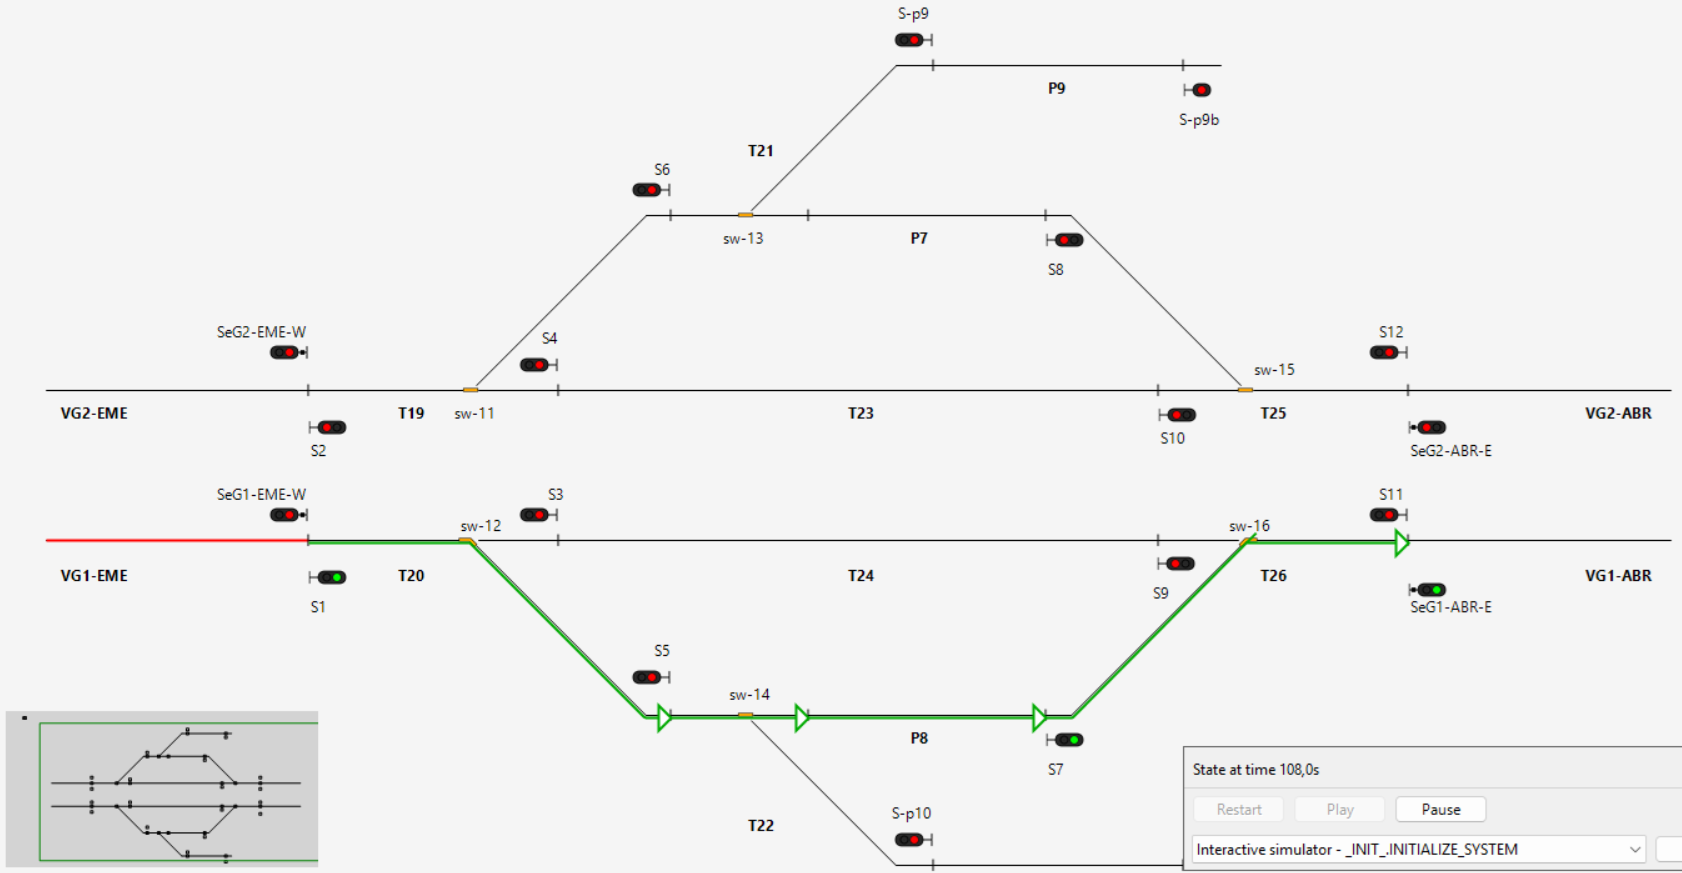
\includegraphics[width=1.0\textwidth,height=4.4cm,keepaspectratio]{../img/simulation_1.png}
    \caption{Simulation at $t = 108.0\,\text{s}$: train approaching Abrial (\code{G-ABR}) from \code{VG1-EME}, with a route set and signals $S_1$ and $S_7$ at proceed towards exit signal \code{SeG1-ABR-E}.}
    \label{fig:sim_abr_approach}
\end{figure}

\begin{figure}[H]
    \centering
    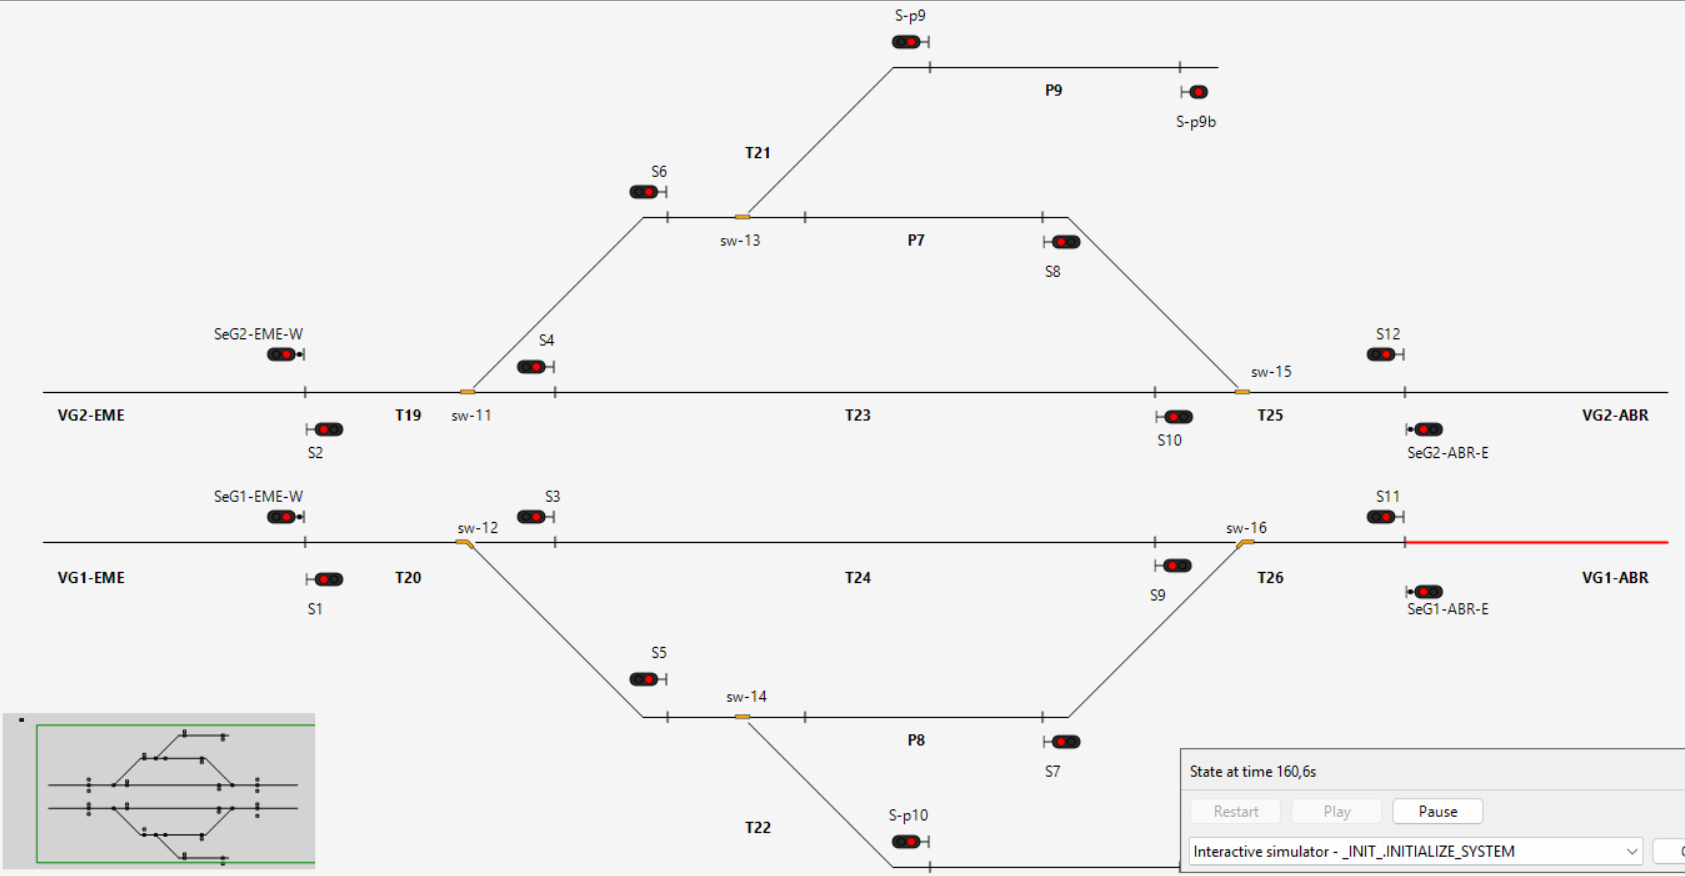
\includegraphics[width=1.0\textwidth,height=4.4cm,keepaspectratio]{../img/simulation_2.png}
    \caption{Simulation at $t = 160.6\,\text{s}$: the train has left Abrial and occupies the line track \code{VG1-ABR} between Abrial and Clarke; the occupancy is shared by both projects.}
    \label{fig:sim_abr_depart}
\end{figure}

\begin{figure}[H]
    \centering
    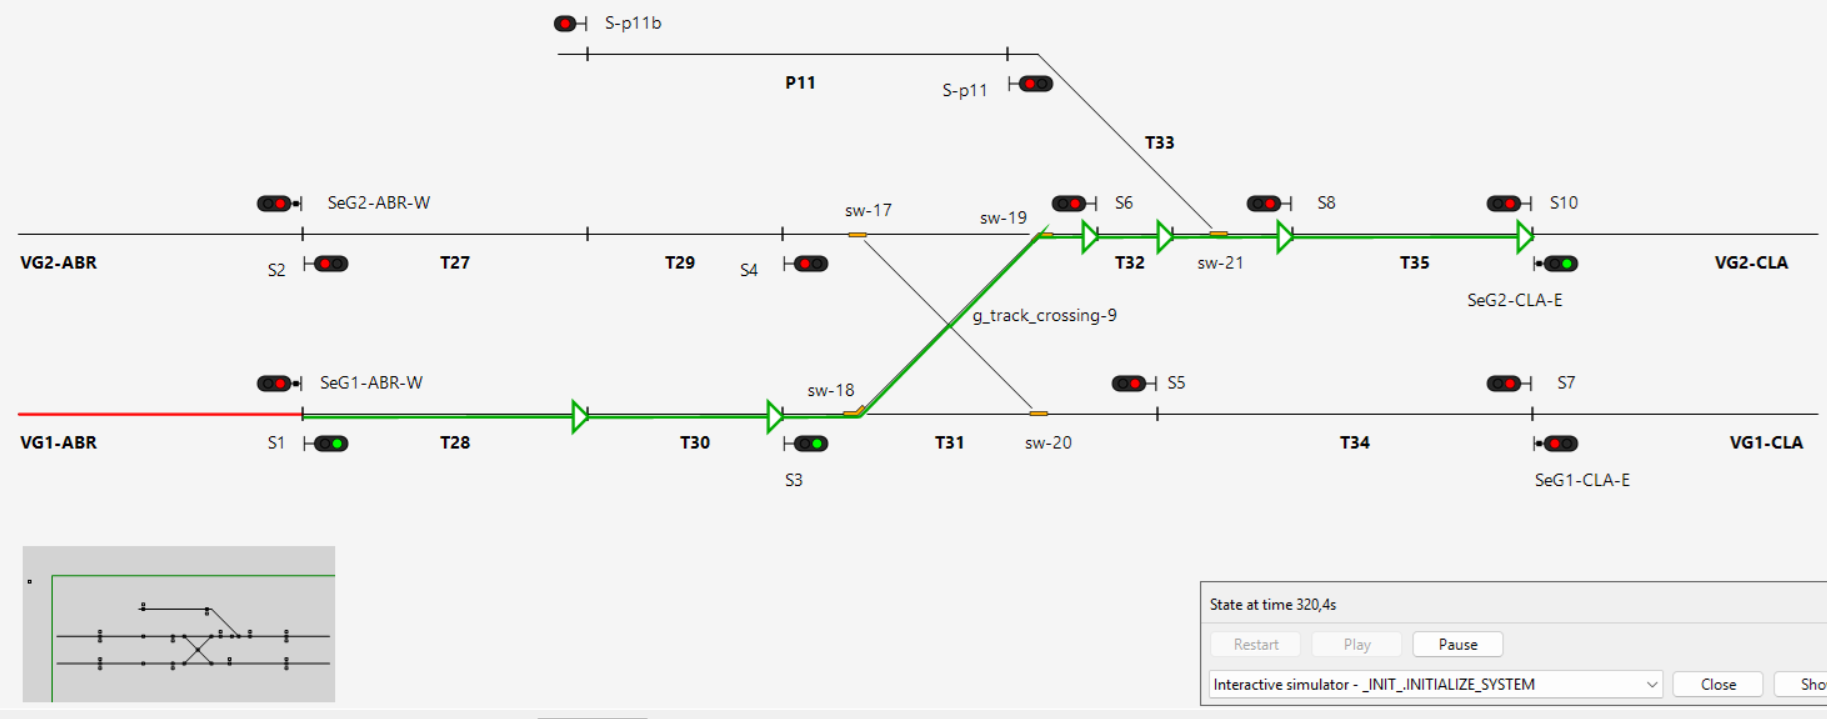
\includegraphics[width=0.96\textwidth,height=4.4cm,keepaspectratio]{../img/simulation_3.png}
    \caption{Simulation at $t = 320.4\,\text{s}$: train entering Clarke (\code{G-CLA}) from \code{VG1-ABR}; entry signal $S_1$ at proceed and route locked across the scissors crossover towards \code{SeG2-CLA-E}.}
    \label{fig:sim_cla_entry}
\end{figure}

One detail of the simulator setup matters beyond the simulation. In \code{EXIT_SIGNAL.tm} the line input starts at true, which is convenient when a station is simulated alone, but it means that a neighbour that is not connected looks like a free line. A real implementation would have to treat a missing or stale message as ``line not free''.

% =========================================================
\section{Verification Results and Limitations}
\label{sec:results}
% =========================================================

\Cref{tab:gss} summarizes the GSS of the delivered package. In the final run the Prover iLock Verifier proves every requirement on the five projects; the counterexamples met along the way are those discussed above.

\begin{table}[tbp]
\centering
\caption{Requirements of the delivered GSS, all proved on the five stations, and their status with respect to the pilot version.}
\label{tab:gss}
\small
\begin{tabularx}{\textwidth}{@{}l Y l l@{}}
\toprule
\textbf{Requirement} & \textbf{Subject} & \textbf{Change} & \textbf{Task} \\
\midrule
\code{GSS_01} (1, 2) & Proceed only with a unique set route, or an end-locked exit signal & unchanged & -- \\
\code{GSS_02} & Sections sharing a track never locked together & formalized & MPS-5, 6 \\
\code{GSS_03} & Switches detected in their route positions & corrected & MPS-3 \\
\code{GSS_04}, \code{GSS_05} & Route tracks clear; flank protection & unchanged & -- \\
\code{GSS_06} & Front protection and line condition & strengthened & MPS-17 \\
\code{GSS_07} & Switch movement lock-out & unchanged & -- \\
\code{GSS_08}, \code{GSS_09} & Ready to release implies occupied, locked & formalized & MPS-7 to 10 \\
\code{GSS_10} & Release only behind a train & formalized, extended & MPS-11, 12, 26 \\
\code{EXIT_1}, \code{EXIT_2} & Line output and exit signal proceed & new & MPS-18 \\
\code{DATACHECK_01}--\code{03} & Placement of exit signals and exit tracks & unchanged & -- \\
\bottomrule
\end{tabularx}
\end{table}

These results should be read for what they are. Each proof concerns one interlocking whose inputs are left free: track occupancy, switch detection, operator requests and the line input can take any value in any cycle. The properties therefore hold whatever the neighbour sends, but they say nothing about the pair. The property that actually matters at a border, that trains are never sent onto a line track from both ends, follows from EXIT 1 and EXIT 2 on both sides only if the link transmits the line output faithfully and without excessive delay. That argument is ours, not the verifier's; checking it formally would require a model that composes two neighbouring interlockings with the communication link.

The interface also has no arbitration. If both stations lock a route towards the same line track within the same communication delay, both see a free line, both lock, and both line outputs then drop. The outcome is safe, because neither start signal can clear without its line input, but both routes stay blocked until one is released manually, which costs at least 30~s. Line block systems used in service usually avoid this situation with an explicit change of traffic direction.

Finally, the GSS only contains safety properties of the form ``something bad never happens''. Several behaviors we care about lie outside it and are covered by tests only: that switches actually move (the defect of \cref{subsec:baseline_defects} went unnoticed by the proofs), that an occupied switch refuses requests (\cref{subsec:tc2}), and that manual release waits 30~s (\cref{subsec:mr_gss}).

% =========================================================
\section{Conclusion}
\label{sec:conclusion}
% =========================================================

During the week we configured the five interlockings of Line G, corrected three defects of the pilot GA, formalized or strengthened five requirements and added two, wrote three test cases, extended the GA with a line block interface and a delayed manual release, and ran the complete line in a connected simulation. All requirements are proved on the five stations and all test cases pass.

The most useful lesson for us concerns the relation between requirements and design. Errors that make a requirement too strong are found at once, because the proof fails. Errors that make it too weak, like the old exit case of Requirement 6, or design errors that make the system do too little, like the switch guard, pass the verifier and were only found by reading the specification critically or by testing. The other lesson is that a manual release forces an exception in a safety requirement, and that such an exception has to be as narrow as possible and paired with a test that checks what the requirement no longer says.

Several extensions follow naturally from this work: the immediate release of routes with no train in their approach area, for which the hook and an approach path class are already in place; a timed requirement for the 30~s delay; a fail-safe default for the line input; and a verification model of two neighbouring interlockings to prove the line block property instead of arguing it.

% =========================================================
% REFERENCES
% =========================================================
\clearpage
\printbibliography[title={References}]

\end{document}
